%%% Folie
{
\small

\begin{frame}{Ausgangslage}
    \parbox{\linewidth}{
        In seiner Standardkonfiguration ist der Raspberry Pi nur begrenzt für größere
        IoT-Anwendungsfälle geeignet, da das mitgelieferte Raspbian-Betriebssystem
        hierfür nicht ausgelegt ist. Dies liegt daran, dass der Raspberry Pi
        hauptsächlich als einfaches Lern- und Experimentiergerät in der Tradition
        früherer Heimcomputer entworfen wurde. Jedoch lässt sich das Betriebssystem
        sehr leicht anpassen oder durch ein maßgeschneidertes Embedded Linux ersetzen.
    }

    \medskip

    \begin{columns}[b,onlytextwidth]
        \column{.48\textwidth}
        \begin{center}
            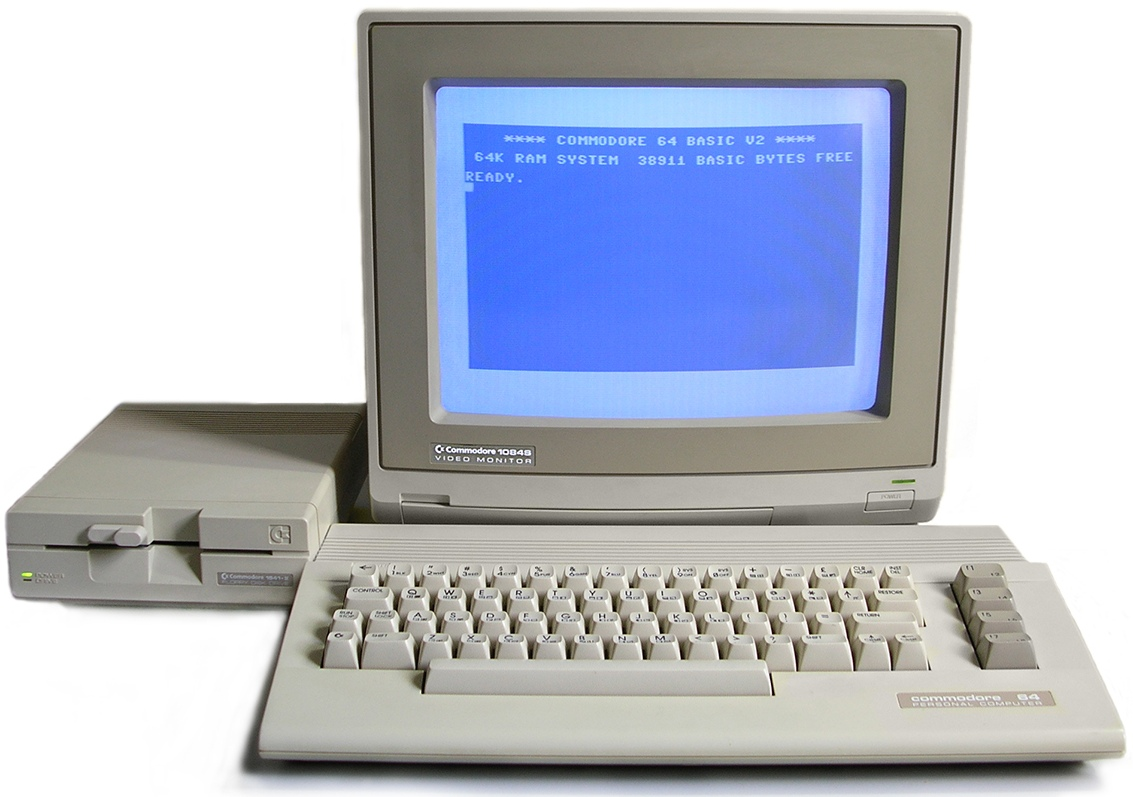
\includegraphics[width=.9\textwidth]{8-linux/img/c64}
        \end{center}
        \parbox{\linewidth}{
            \footnotesize
            \textbf{Commodore 64:}
            Beispiel für einen weit verbreiteten Heimcomputer der 1980er-Jahre
            mit eingebautem BASIC-Interpreter
        }

        \column{.48\textwidth}
        \begin{center}
            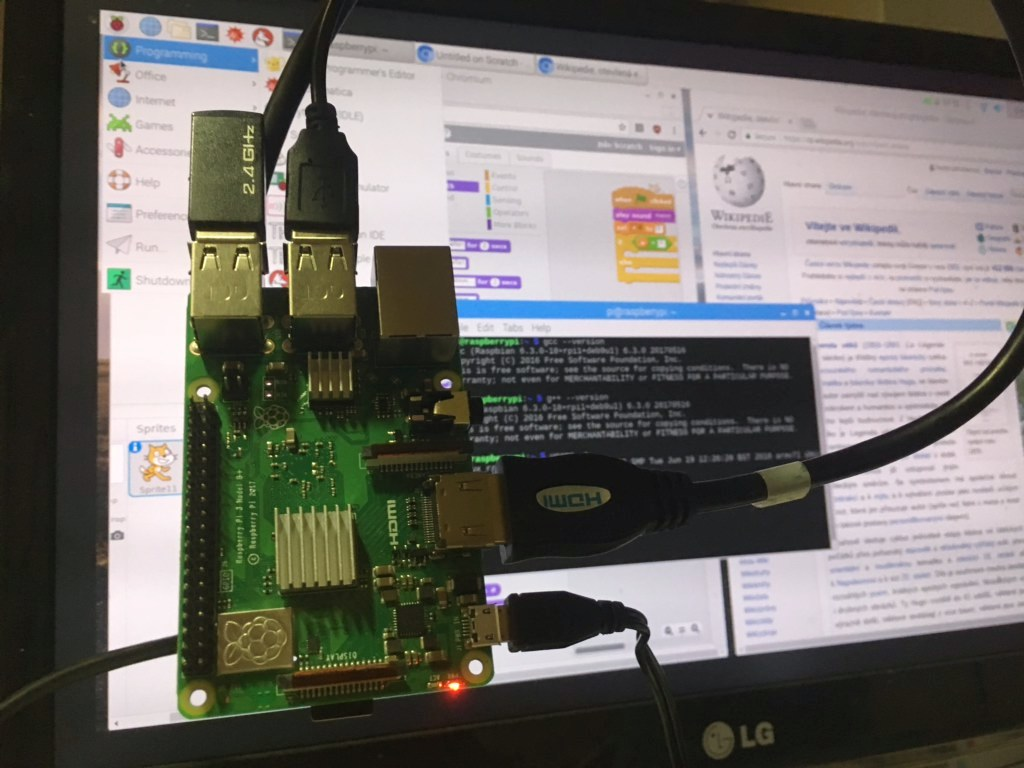
\includegraphics[width=.85\textwidth]{8-linux/img/raspi}
        \end{center}
        \parbox{\linewidth}{
            \footnotesize
            \textbf{Rasbperry Pi:} Modermer Versuch, einen Computer zum
            Experimentieren und Programmieren Lernen zu bauen
        }
    \end{columns}
\end{frame}
}

%%% Folie
\begin{frame}{Lernziele}
    \begin{block}{Linux auf dem Raspberry Pi}
        \begin{itemize}
            \item Linux im Vergleich zu anderen Betriebssystemen einordnen können
            \item Den typischen Aufbau eines Linux-Systems beschreiben können
            \item Den Filesystem Hierarchy Standard kennen und verstehen
            \item Den Bootvorgang des Raspberry Pi vollständig erklären können
            \item Raspbian für eigene kleine Projekte konfigurieren können
        \end{itemize}
    \end{block}

    \begin{block}{Erstellung eigener Linux-Systeme}
        \begin{itemize}
            \item Die Vorgehensweise beim Bau eigener Images kennen und verstehen
            \item Ein geeignetes Toolkit zum Bau von Linux-Systemen auswählen können
            \item Eigene Linux Images mit den vorgestellten Toolkits erzeugen können
            \item Eigene Programme in die selbst erstellten Images integrieren können
        \end{itemize}
    \end{block}
\end{frame}

%%% Folie
\begin{frame}{Inhaltsübersicht}
    \tikzset{
        MyTitle/.style={
            align=left,
            text=blue!65!purple,    % 65% blue, 35% purple
            anchor=north west,
            font=\large,
        },
        MyNode1/.style={
            below=2pt,
            align=left,
            anchor=north west,
            font=\footnotesize
        },
        MyNode2/.style={
            above=2pt,
            align=left,
            anchor=south west,
            font=\footnotesize
        },
        MyNumber/.style={
            text=white,
            font=\scriptsize
        }
    }

    % Vgl. https://tex.stackexchange.com/a/18201
    \pgfdeclarelayer{bg}
    \pgfsetlayers{bg, main}

    \begin{columns}
        \column{\dimexpr\paperwidth-1.4cm}
        \begin{tikzpicture}
            % Linux auf dem Rasbperry Pi
            \node[MyTitle] at (0,0) {Linux auf dem Rasbperry Pi};
            \filldraw[fill=darkred]
                ( 0,-0.6) circle(4pt) node(pi-1){} node[MyNumber]{1}  node[MyNode1]{Anforderungen an \\ das Betriebssystem}
                ( 4,-0.6) circle(4pt) node(pi-2){} node[MyNumber]{2}  node[MyNode1]{Linux im Vergleich zu \\ anderen Betriebssystemen}
                ( 8,-0.6) circle(4pt) node(pi-3){} node[MyNumber]{3}  node[MyNode1]{Typischer Aufbau \\ eines Linux-Systems};
            \filldraw[fill=gray!50]
                (11,-0.6) circle(4pt) node(pi-tr){}
                (11,-2.6) circle(4pt) node(pi-br){};
            \filldraw[fill=darkred]
                ( 8,-2.6) circle(4pt) node(pi-4){} node[MyNumber]{4}  node[MyNode2]{Der Bootvorgang des \\ Raspberry Pi im Detail}
                ( 4,-2.6) circle(4pt) node(pi-5){} node[MyNumber]{5}  node[MyNode2]{Benutzer- und Netzwerk- \\ konfiguration in Raspbian}
                ( 0,-2.6) circle(4pt) node(pi-6){} node[MyNumber]{6}  node[MyNode2]{Konfiguration des \\ Raspbian-Startvorgangs};

            % Erstellung eigener Linux-Systeme
            \node[MyTitle] at (0,-3.4) {Erstellung eigener Linux-Systeme};
            \filldraw[fill=darkred]
                ( 0,-4.0) circle(4pt) node(mk-1){} node[MyNumber]{7}  node[MyNode1]{Generelles Vorgehen beim \\ Bau eines Firmware-Images}
                ( 4,-4.0) circle(4pt) node(mk-2){} node[MyNumber]{8}  node[MyNode1]{Vergleich verschiedener \\ Baukästen für Linux}
                ( 8,-4.0) circle(4pt) node(mk-3){} node[MyNumber]{9}  node[MyNode1]{Linux-Images bauen \\ mit Rasbperry Pi Gen};
            \filldraw[fill=gray!50]
                (11,-4.0) circle(4pt) node(mk-tr){}
                (11,-6.0) circle(4pt) node(mk-br){};
            \filldraw[fill=darkred]
                ( 8,-6.0) circle(4pt) node(mk-4){} node[MyNumber]{10} node[MyNode2]{Linux-Images bauen \\ mit Buildroot}
                ( 4,-6.0) circle(4pt) node(mk-5){} node[MyNumber]{11} node[MyNode2]{Linux-Images bauen \\ mit Ubuntu Core}
                ( 0,-6.0) circle(4pt) node(mk-6){} node[MyNumber]{12} node[MyNode2]{Fazit und Ausblick};

            % Verbindungslinien
            \begin{pgfonlayer}{bg}
                \draw (pi-1) -- (pi-2) -- (pi-3) -- (pi-tr) -- (pi-br) -- (pi-4) -- (pi-5) -- (pi-6);
                \draw[gray, densely dashed] (pi-6) -- (mk-1);
                \draw (mk-1) -- (mk-2) -- (mk-3) -- (mk-tr) -- (mk-br) -- (mk-4) -- (mk-5) -- (mk-6);
            \end{pgfonlayer}
        \end{tikzpicture}
    \end{columns}
\end{frame}

%-------------------------------------------------------------------------------
\section{Linux auf dem Raspberry Pi}
%-------------------------------------------------------------------------------

%%% Folie
% TODO: Anfordderungen besser und vollständiger formulieren?
{
\small
\setlength{\leftmargini}{1.2em}

\begin{frame}{Anforderungen an das Betriebssystem}
    \begin{columns}[T]
        \column{.33\textwidth}
        \begin{block}{Embedded Devices}
        \end{block}

        \column{.33\textwidth}
        \begin{block}{IoT-Devices}
        \end{block}

        \column{.33\textwidth}
        \begin{block}{Sonstige Computer}
        \end{block}
    \end{columns}

    \begin{columns}[T]
        % Embedded Devices
        \column{.33\textwidth}
        \begin{itemize}
            \item Verwaltung der Hardwareressourcen
            \item Unterstützung von Multi-Tasking
            \item Datenaustausch innerhalb des Systems
        \end{itemize}

        % IoT-Devices
        \column{.33\textwidth}
        \begin{itemize}
            \item Datenaustausch über das Internet
            \item Zugriffsbeschränkungen, Firewalls, Sicherheit
            \item Lokale Datenhaltung
            \item Zentrales Monitoring
        \end{itemize}

        % Sonstige Computer
        \column{.33\textwidth}
        \begin{itemize}
            \item Breite Hardwareunterstützung
            \item Mehrbenutzerbetrieb
            \item Flexibilität und Konfigurierbarkeit
            \item Umfangreiche Anwendungsfunktionen
        \end{itemize}
    \end{columns}

    \vfill

    \begin{columns}[T]
        % Embedded Devices
        \column{.33\textwidth}
        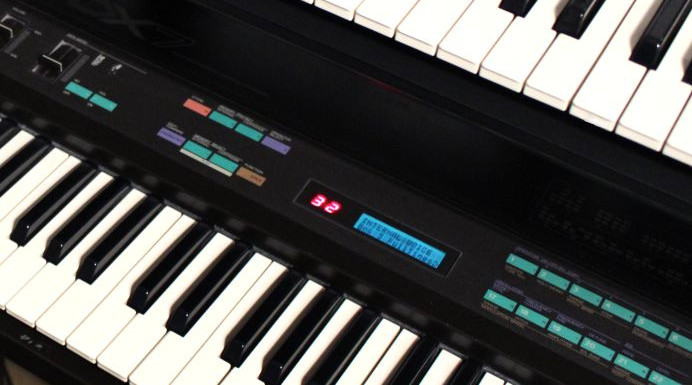
\includegraphics[width=\textwidth]{8-linux/img/os-embedded}

        % IoT-Devices
        \column{.33\textwidth}
        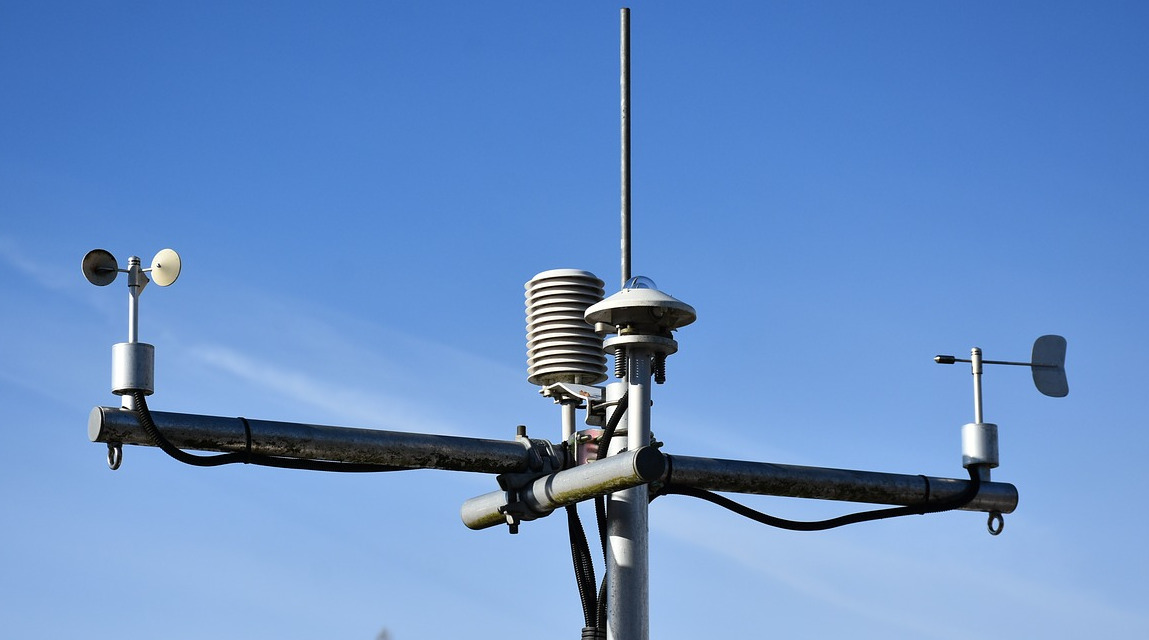
\includegraphics[width=\textwidth]{8-linux/img/os-iot}

        % Sonstige Computer
        \column{.33\textwidth}
        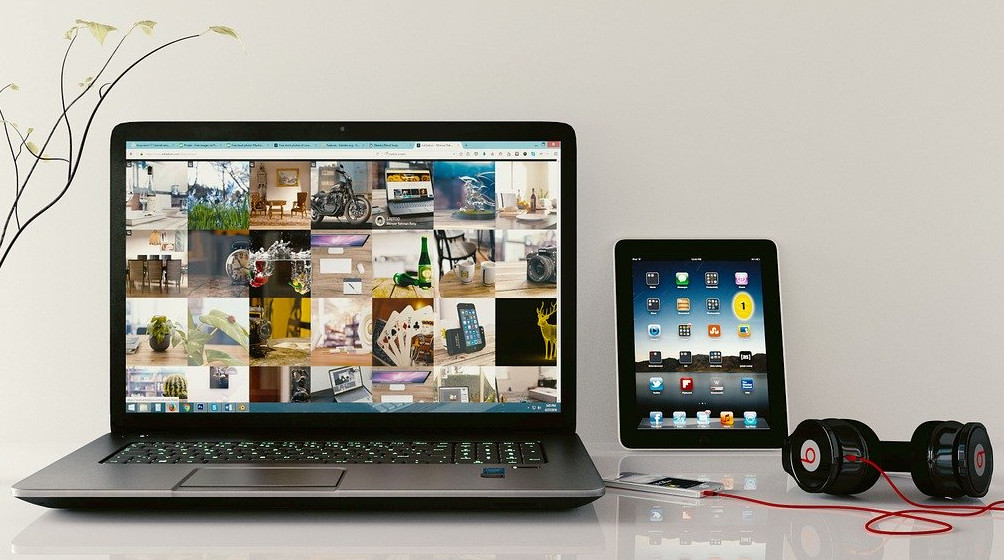
\includegraphics[width=\textwidth]{8-linux/img/os-workstation}
    \end{columns}
\end{frame}
}

%%% Folie
\begin{frame}{Linux im Vergleich zu anderen Betriebssystemen}
    TODO
\end{frame}

%%% Folie
{
\footnotesize

\begin{frame}[allowframebreaks]{Typischer Aufbau eines Linux-Systems}
    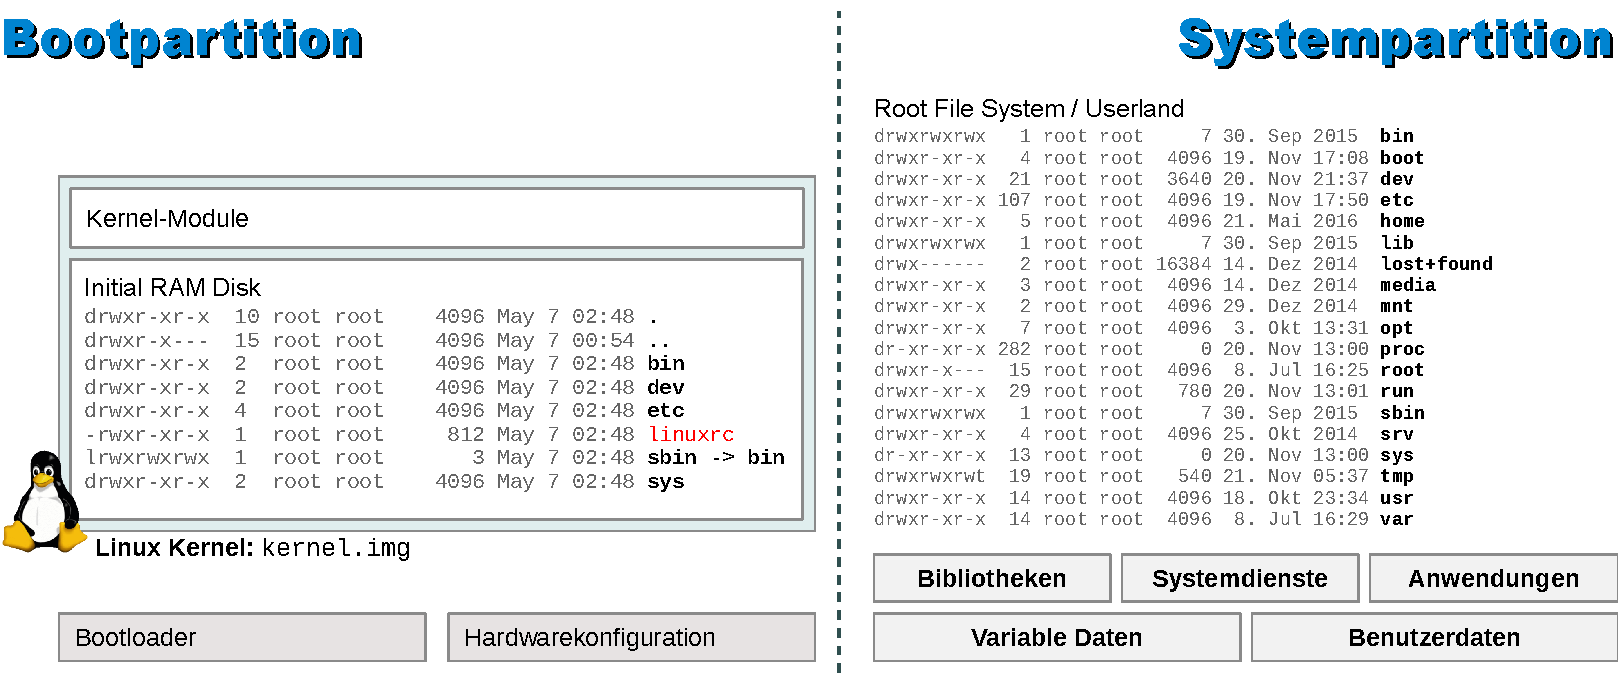
\includegraphics[width=\textwidth]{8-linux/img/linux-aufbau}
    \smallskip

    \parbox{\linewidth}{
        Linux-basierte Betriebssysteme setzen sich immer aus einem \textbf{Kernel}
        und dem \textbf{Userland} zusammen. Wie für eingebettete Systeme typisch,
        befinden sich beide beim Raspberry Pi in getrennten Partitionen, wobei die
        Boot-Partition zusätzlich noch den Bootloader und Konfigurationsdateien zur
        Initialisierung der Hardware beinhaltet.
    }

    {
        \bigskip
        \scriptsize

        \begin{columns}[T, onlytextwidth]
            \column{.49\textwidth}
            \parbox{\linewidth}{
                \textbf{Systemdienste:} Systemnahe Programme, Hintergrundjobs und
                Serverprogramme
            }

            \column{.49\textwidth}
            \parbox{\linewidth}{
                \textbf{Anwendungen:} Zusätzliche Anwendungsprogramme, die keine
                Systemfunktionen im engeren Sinne erfüllen
            }
        \end{columns}

        \medskip

        \begin{columns}[T, onlytextwidth]
            \column{.49\textwidth}
            \parbox{\linewidth}{
                \textbf{Variable Daten:} Während der Benutzung des Systems automatisch
                anfallende Daten
            }

            \column{.49\textwidth}
            \parbox{\linewidth}{
                \textbf{Benutzerdaten:} Durch den Endanwender erzeugte und verwaltete
                Daten
            }
        \end{columns}
    }

    \framebreak
    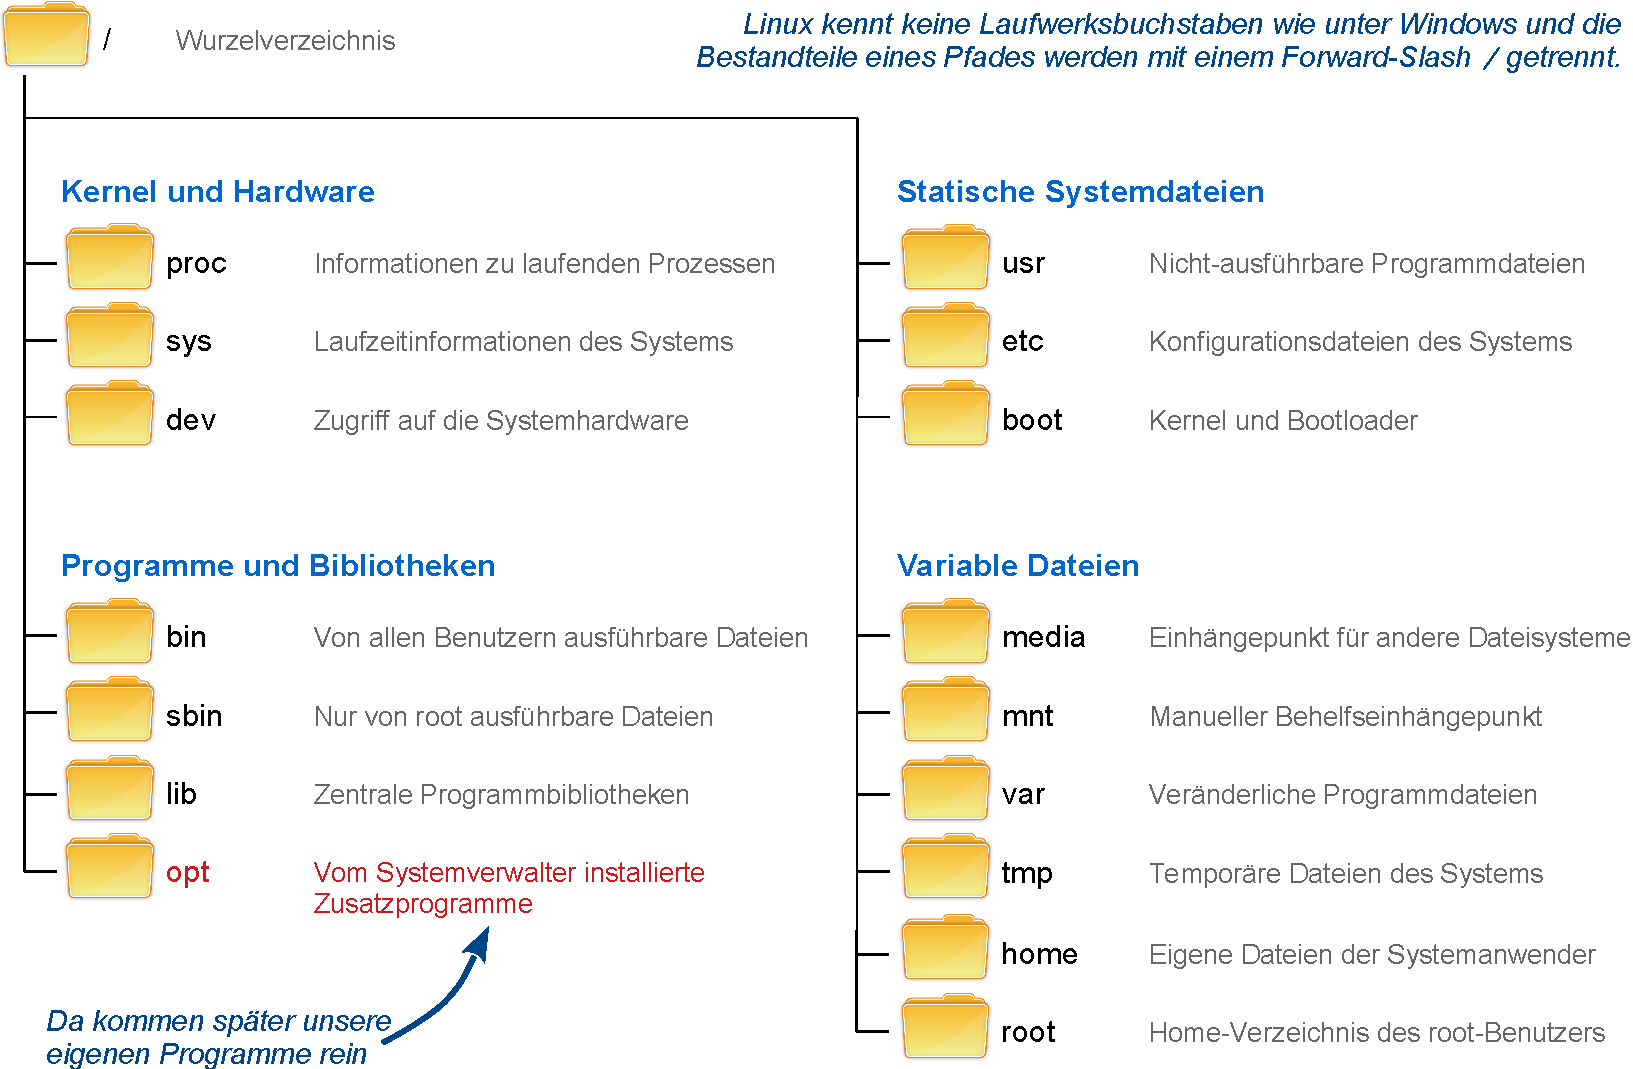
\includegraphics[width=\textwidth]{8-linux/img/fhs-verzeichnisse}
\end{frame}
}

%%% Folie
\begin{frame}{Der Bootvorgang des Raspberry Pi im Detail}
    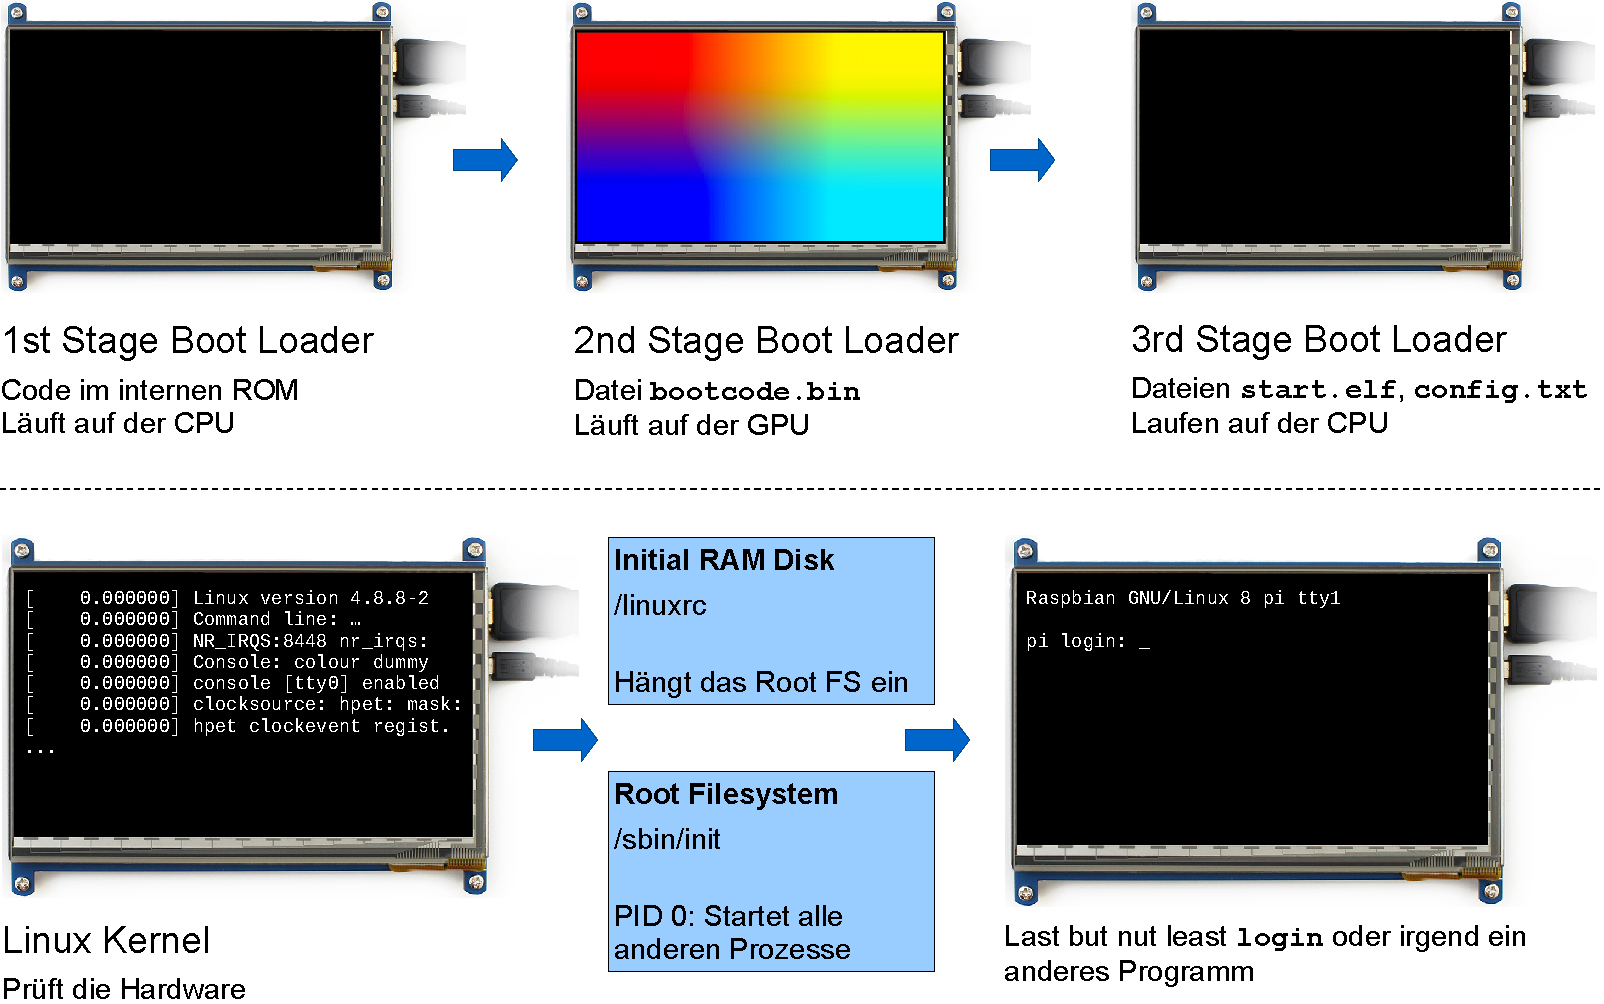
\includegraphics[width=\textwidth]{8-linux/img/pi-bootvorgang}
\end{frame}

%%% Folie
\begin{frame}{Benutzer- und Netzwerkkonfiguration in Raspbian}
    TODO
\end{frame}

%%% Folie
\begin{frame}{Konfiguration des Raspbian-Startvorgangs}
    TODO
\end{frame}

%-------------------------------------------------------------------------------
\section{Erstellung eigener Linux-Systeme}
%-------------------------------------------------------------------------------

%%% Folie
\begin{frame}{Generelles Vorgehen beim Bau eines Firmware-Images}
    TODO
\end{frame}

%%% Folie
\begin{frame}{Vergleich verschiedener Baukästen für Linux}
    TODO
\end{frame}

%%% Folie
\begin{frame}{Linux-Images bauen mit Raspberry Pi Gen}
    TODO
\end{frame}

%%% Folie
\begin{frame}{Linux-Images bauen mit Buildroot}
    TODO
\end{frame}

%%% Folie
\begin{frame}{Linux-Images bauen mit Ubuntu Core}
    TODO
\end{frame}

%%% Folie
\begin{frame}{Fazit und Ausblick}
    TODO
\end{frame}

